\chapter{Introduction \& Summary}

%Provide a short summary of the whole PhD thesis:
% -Introduction to QC & CQED
% -Building Blocks of Superconducting Quantum Processors
% -Realization of a Two-Transmon QP
% -Tune-Up & Characterization of the Universal Two-Qubit Gate
% -Grover's Algorithm: Introduction & Background
% -Implementation on the Two-Qubit Processor
% -Design of a Scalable QC Architecture



\section{Quantum Computing with Superconducting Circuits}

%
\begin{figure}
\centering 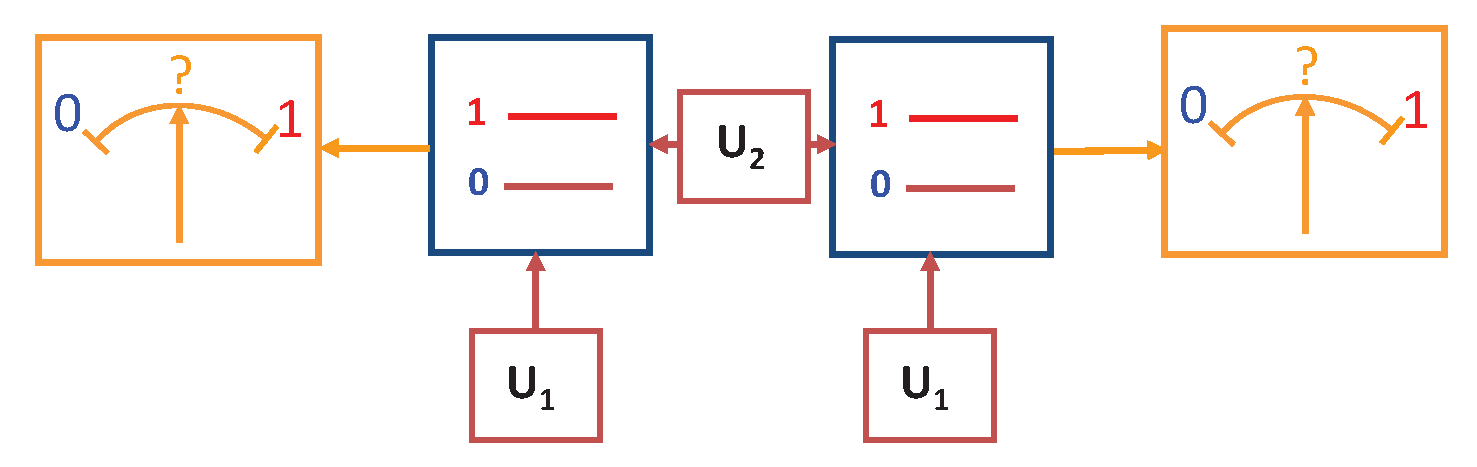
\includegraphics[width=0.8\textwidth]{./material/papers/grover/submission1/Fig1}
\caption[Blueprint of a {}``canonical'' two-qubit quantum processor]{The blueprint of a {}``canonical'' two-qubit quantum processor.
The two qubits can be individually manipulated ($U_{1}$) and a by
a universal two-qubit gate $U_{2}$ can be applied to them. Each of
the qubits can be read out individually.}


\label{fig:qubit_processor_blueprint} %
\end{figure}


This thesis presents experiments performed with a superconducting
two-qubit quantum processor. The main goal of this work was to demonstrate
a possible quantum computing architecture based on superconducting
qubits that follows the canonical blueprint of a quantum processor
as sketched in fig. \ref{fig:qubit_processor_blueprint},
in accordance with the five criteria formulated by DiVincenzo\citep{divincenzo_physical_2000}.
By this definition, a universal quantum computer is a register of
well-defined quantum bits (1) with long coherence times (2),
on which one can implement any unitary evolution using a universal
set of quantum gates (3), fitted with individual high fidelity readout
of each qubit (4) and with qubit reset in their ground state (5). Implementing this allegedly simple list of requirements
in a system of superconducting qubits has been a major research challenge
during the last decade, and is part of more general line of research
on superconducting quantum circuits briefly summarized below.

%
\begin{figure}[ht!]
 \centering 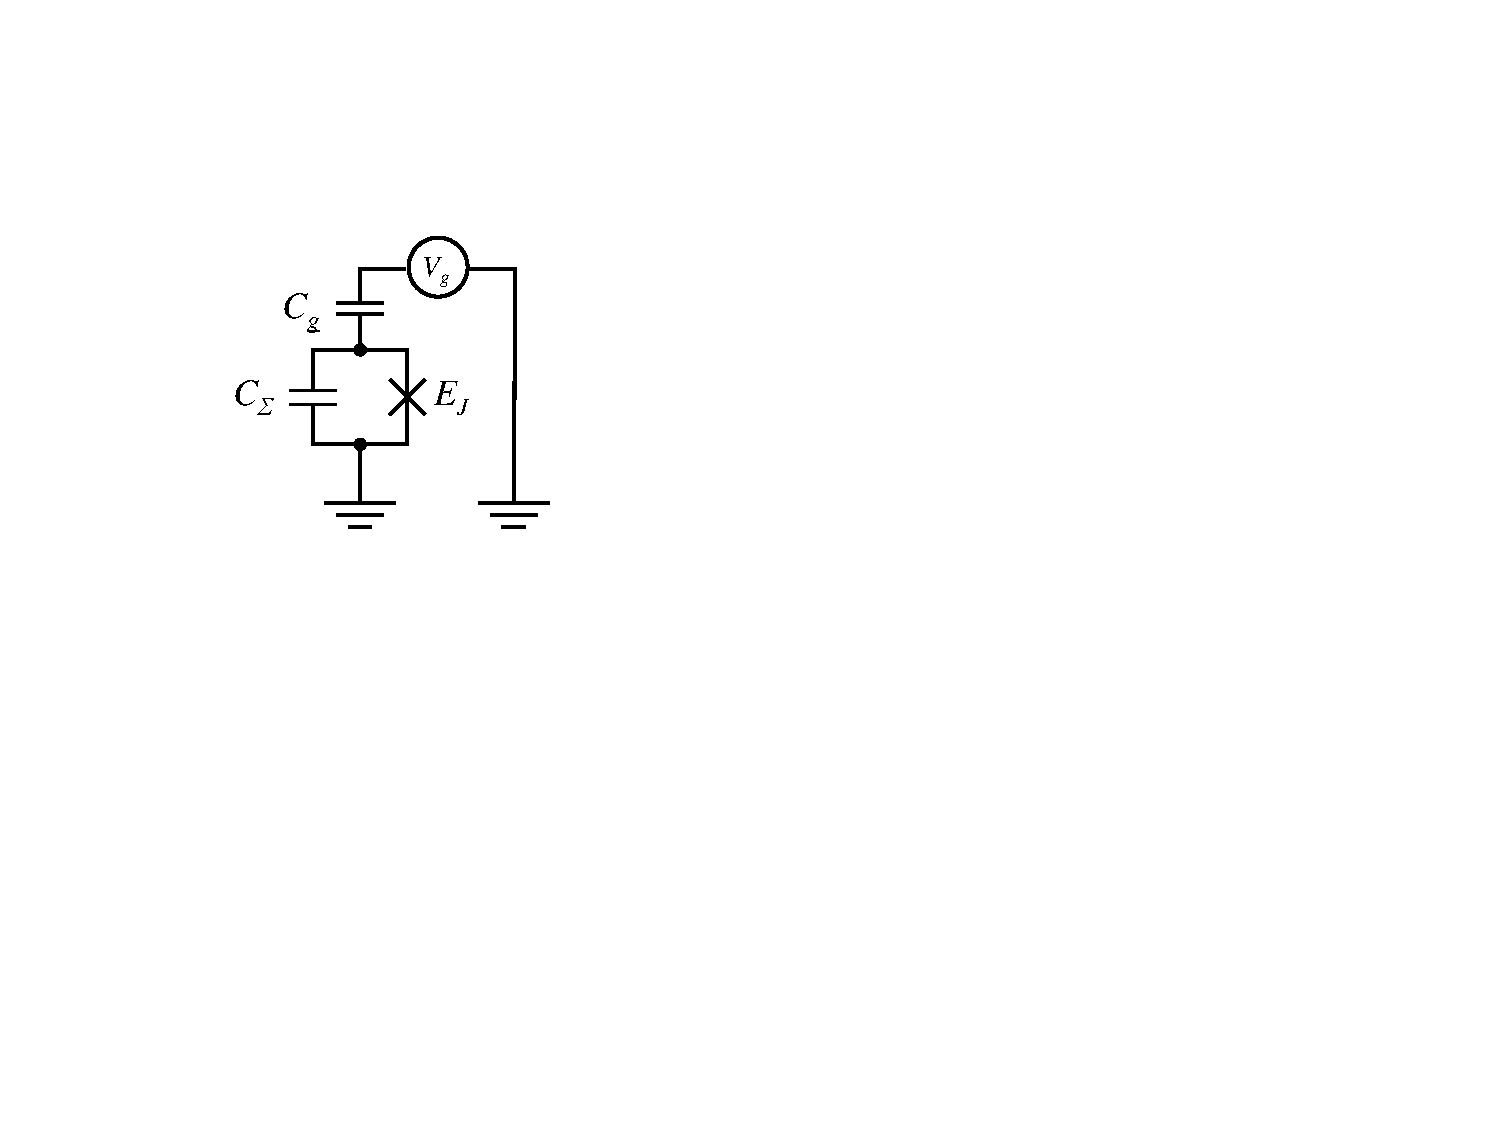
\includegraphics[width=10cm]{./material/figures/introduction/cooper_pair_box_simple}
\caption[]{a) The schematic of the simple Cooper pair box (CPB) circuit, consisting
of a capacitor in parallel with a Josephson junction and capacitively
coupled to a voltage source. b)The same schematic using the simplified
circuit symbol for the CPB Josephson junction.}


\label{fig:cooper_pair_box_simple} %
\end{figure}



\subsection{Context of this thesis work: 25 years of superconducting
quantum circuits}

The observation of quantum tunneling in a current-biased
Josephson junction switching out of its zero-voltage
state by Devoret et. al. \citep{devoret_measurements_1985,martinis_energy-level_1985},
first demonstrated that a collective electrical variable
such as the superconducting phase difference across a Josephson junction (or the conjugated variable, i.e. the number of Cooper
pairs that crossed it) can exhibit quantum properties. Then,
the observation of microwave induced transitions between the quantum
states of the junction by Martinis et. al. \citep{martinis_energy-level_1985} further
confirmed the quantum nature of this degree of freedom (See also \cite{martinis_energy-level_1985,martinis_experimental_1987,clarke_quantum_1988}).
A somewhat simpler quantum electrical circuit called the single Cooper
Pair Box (CPB), made of a Josephson junction in series
with a gate capacitor and a voltage source as shown in fig.
\ref{fig:cooper_pair_box_simple}, was later developed in the Quantronics
group during the 1990s \citep{bouchiat_quantum_1998},
and its ground state was mapped. With this electrical
circuit, Nakamura et. al. \citep{nakamura_coherent_1999} did the first superconducting
qubit experiment by demonstrating coherent oscillations between its
ground and first excited eigenstates. Although the achieved coherence
time was quite short, in the 5-10 ns range, this result attracted
a huge interest and triggered the active development of research on
superconducting quantum bits.

\smallskip

In the years after, several types of superconducting qubits were proposed
using Josephson junctions in different configurations. Different regimes,
in which the quantum state of the junctions ranges from almost Cooper
pair number states to phase states, were realized. Let us cite here
the flux qubit \citep{mooij_josephson_1999, chiorescu_coherent_2003}
and the phase qubit\citep{martinis_rabi_2002}, which were very
successful qubits in many aspects. On the side of Cooper Pair Boxes,
the Quantronics group made a significant progress by operating a
new circuit called the \textit{Quantronium} Vion et. al. \citep{vion_manipulating_2002},
fitted with a strategy for fighting dephasing due to the noise of
the electrical control parameters, and with a single-shot
readout (although with limited fidelity). The robustness of the quantronium
arises from its operation at a so-called sweet spot where the qubit
frequency is stationary respectively to variations of all
the control parameters. The improved coherence of
the quantonium allowed to perform all the basic manipulations possible
on spins and more generally on two level systems \citep{collin_nmr-like_2004}.
Shortly after, another CPB design, inspired from
cavity-QED, was developed at Yale by Wallraff et. al. \citep{wallraff_strong_2004}.
In this so-called circuit-QED (CQED) design, the
CPB, embedded in a microwave resonator, can be thought as an artificial
atom in a resonant cavity. The qubit readout is obtained
dispersively, i.e. through the cavity pull of the resonator frequency
controlled by the qubit state. This small frequency change results
in a small phase change of a resonant microwave pulse, which yields
after sufficient repetition the probability of the two qubit states
\citep{blais_cavity_2004}.

\smallskip{}


Another great bonus of CQED is that the electromagnetic
environment in which the qubit relaxes its energy consists of a microwave
resonator with a well controlled impedance. The modern
version of the Cooper Pair Box called \textit{Transmon}, follows this
design with an extra feature that makes it insensitive to the charge
noise that plagues single electron and single Cooper Pair devices.
This feature consists in placing the Cooper Pair
Box in the phase regime by adding an extra capacitance in
parrallel with the junction: the qubit frequency is then
totally insensitive to the gate charge, and hence to the charge noise.
This new design, that however still leaves sufficient anharmonicity
to operate the device as a qubit and allows to drive it, yielded a
sizeable improvement in coherence times, qubit robustness and usability.
The CQED concept was thus rapidly extended to flux and phase qubits.

In 2010, a new type of CQED architecture has been
developed by Paik et. al. \citep{paik_observation_2011} that combines Transmon
qubits with 3D cavities instead of CPW resonators, resulting again
in an impressive increase of qubit coherence times of up to two orders
of magnitude, with reported qubit relaxation times
and coherence times approaching $100\;\mu\mathrm{s}$.
Very recently, these drastically improved coherence times have made
possible the realization of elemental quantum feedback and error correction
schemes with these systems\citep{vijay_quantum_2012}.

\smallskip

The progress achieved during the last decade on the
Cooper Pair Box and on the phase qubits has benefited to quantum processors.
So far, superconducting CQED processors with up to three qubits have
been realized and two- and three-qubit quantum gates \citep{fedorov_implementation_2011},
multi-qubit entanglement \citep{dicarlo_preparation_2010} and simple
quantum algorithms \citep{dicarlo_demonstration_2009} as well as
quantum error correction  \citep{reed_realization_2011} have recently
been demonstrated.

\subsection{This Thesis Work}

At the beginning of this thesis work, CQED processors
having demonstrated quantum algorithms did not follow all the rules
established by DiVincenzo \citep{divincenzo_physical_2000}; in other words, they
did not follow the canonical blueprint able to demonstrate quantum
speed-up: they were all fitted with a joint readout, which allows
to measure the average value of a collective variable of the qubit
register, but not each qubit individually. By repeating a given sequence
of gates a large number of times, one can nevertheless determine the
quantum state of the qubit register at different steps of the algorithm
being run. Since the whole interest of quantum computing is precisely
to perform computational tasks more efficiently than with a classical
processors, it was essential, in our mind, to demonstrate the quantum
speed-up expected from quantum algorithms with a c-QED quantum processor
fitted with individual single shot and non-demolishing (QND) readouts
for each qubit. Such a high fidelity single-shot readout had been
developped for a single transmon during a previous thesis in the Quantronics
group\citep{mallet_single-shot_2009,palacios-laloy_superconducting_2010}, and it was natural to use it in the present work.

\smallskip

This thesis discusses therefore the realization of
a superconducting two-qubit processor based on Transmon qubits fitted
with individual single-shot readouts. With this processor, we implement
elementary one- and two-qubit quantum operations and use it to run
a simple quantum algorithm that demonstrates probabilistic quantum
speed-up: the Grover search algorithm. Finally, we discuss the realization
of a four-qubit quantum processor using a more scalable approach that
could possibly be extended to an even larger number of qubits.

Note that during this thesis work, quantum speed-up
was also demonstrated for the Deutsch-Josza algorithm with a phase
qubit processor using individual single-shot and destructive readouts
\citep{yamamoto_quantum_2010}.


\section{Realizing a Two-Qubit Quantum Processor}

%
\begin{figure}[ht!]
 \centering 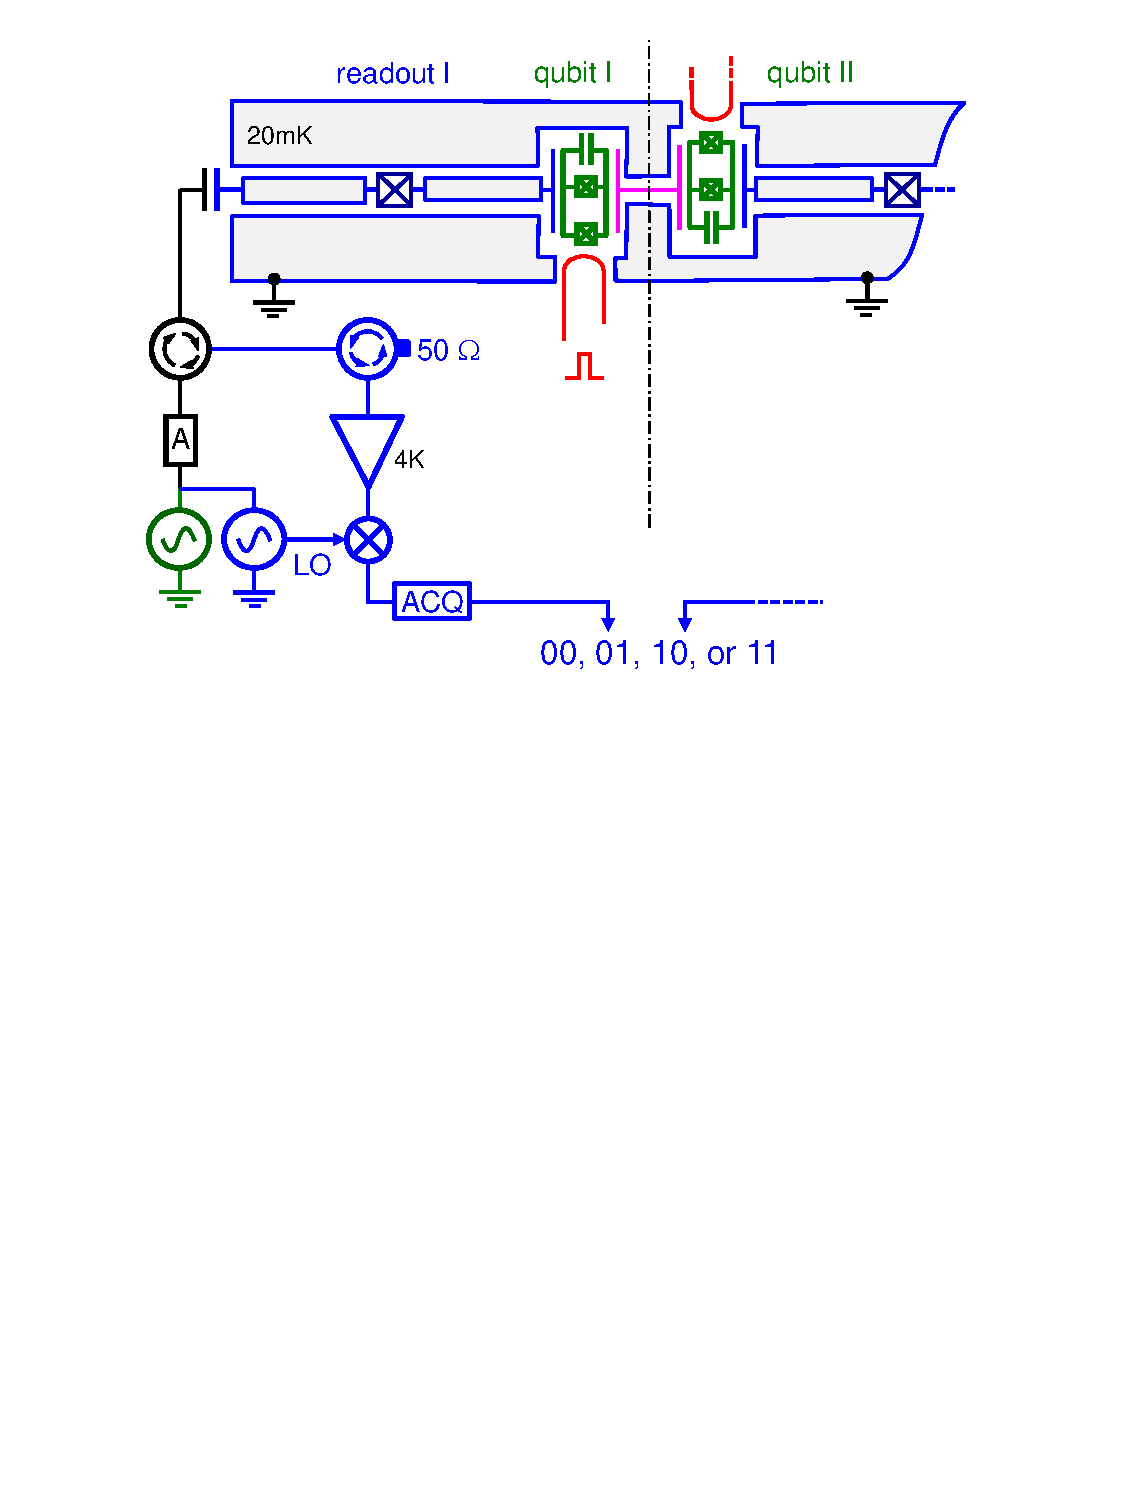
\includegraphics[width=0.75\textwidth]{./material/papers/grover/figures/2_qubit_processor_schematic}
\caption[Circuit schematic of the realized two-qubit processor]{Circuit schematic of the two-qubit processor realized in this thesis work, showing the two qubits (in green) coupled by
a fixed capacitor (in purple), as well as the fast flux lines (in
red) used to tune the qubit frequencies and the qubit readouts (in
blue). Each qubit is embedded in its own nonlinear readout resonator
and can be driven and read out by microwave reflectometry through an individual microwave line.}


\label{fig:two_qubit_processor_schematic} %
\end{figure}


The quantum processor implemented in this work is shown in Fig. \ref{fig:two_qubit_processor_schematic}.
It consists of two superconducting quantum bits of the Transmon type,
each equipped with its own drive and readout circuit. In order to
obtain a high fidelity single-shot readout of the qubit register,
we used the Josephson Bifurcation Amplifier (JBA) readout method first
developed in the team of Michel Devoret at Yale for the quantronium
qubit \citep{siddiqi_rf-driven_2004,vijay_invited_2009}. This method
had indeed already been successfully adapted to the transmon, and
yielded a 93 \% readout fidelity \citep{mallet_single-shot_2009}.
The qubit readout is realized using a nonlinear coplanar-waveguide
resonator that serves as a \textit{cavity bifurcation amplifier} (CBA)\citep{siddiqi_dispersive_2006,vijay_invited_2009}
and allows a single-shot readout of the qubit state \citep{mallet_single-shot_2009}.
Each qubit can be manipulated by driving it with microwave pulses
through its readout resonator, allowing for robust and fast single-qubit
operations. The qubit frequencies can be tuned individually using
fast flux lines, allowing us to change the frequency of each qubit
over a range of several GHz. The coupling between the two qubits is
realized through a fixed capacitance that connects the two top-electrodes
of the Transmons and implements a fixed $\sigma_{xx}$-type qubit-qubit
coupling. This coupling allows us to generate entangled two-qubit
states and to implement a two-qubit gate. We use this simple processor
to generate entangled two-qubit states, test the Bell inequality,
implement a universal two-qubit gate and perform a simple quantum
algorithm that demonstrates quantum speed-up, as will be discussed
in the following sections.


\section{Demonstrating Simultaneous Single-Shot Readout}

%
\begin{figure}[ht!]
 \centering \includegraphics[width=0.5\textwidth]{"./material/papers/grover/figures/s curves"}
\includegraphics[width=0.43\textwidth]{"./data/ct5/2011_04_21 - grover and tomo/good_data/readout only"}
\caption[Switching probabilities of the two qubit readouts as a function of
the readout excitation power]{a) Switching probabilities of the two readout resonators
as a function of the readout drive power at a fixed driving frequency.
The measurement is performed after preparing the qubits in the states
${\color{blue}{\ket{0}}}$, ${\color{red}{\ket{1}}}$ and ${\color{brown}{\ket{2}}}$.
The readout contrast is given as the difference in probability between
the curves corresponding to the states ${\color{blue}{\ket{0}}}$
and ${\color{red}{\ket{1}}}$ or ${\color{brown}{\ket{2}}}$, respectively.
The highest contrasts of 88 and 89 \% are achieved when the qubit
is shelved from state${\color{red}{\ket{1}}}$ to ${\color{brown}{\ket{2}}}$.
b)Readout matrix of the two-qubit system, giving
the probabilities to obtain the different outcomes ij after having
prepared the register in the different computational basis states
$\left|kl\right\rangle $.}


\label{fig:qubit_readout_characteristics} %
\end{figure}


For readout, each qubit is capacitively coupled to
a coplanar waveguide resonator made nonlinear by placing a Josephson
junction in its central conductor. We exploit the frequency pull of
the bifurcation transition that occurs in such a resonator when driven
at a suitable frequency and power to map the qubit
states on the bifurcated and non bifurcated cavity states, which are
then discriminated by reflectometry. Here, the hysteretic
character of the bifurcation transition allows to reduce the measuring
power, to latch the cavity state, and to measure it without being
affected by subsequent qubit relaxation. The state of the resonator
can thus be determined reliably without being limited by qubit relaxation,
thereby providing a high-fidelity single-shot qubit readout. Contrary
to previous CQED processors, our processor is fitted with individual
readout, and a simultaneous readout of the full two-qubit register
is possible, as requested by the DiVincenzo criteria. For single-qubit
CBA readouts, readout fidelities up to 93 \% have been achieved
\citep{mallet_single-shot_2009} by shelving the first excited state
of the transmon (qubit state $\left|1\right\rangle $ ) to the higher
excited state $\left|2\right\rangle $. However, due to the higher
complexity and design constraints of our system, only 83-89 \% fidelity
has been achieved for the processor presented here. The full characterization
of the readout of our processor is shown in fig.
\ref{fig:qubit_readout_characteristics}. Figure \ref{fig:qubit_readout_characteristics}a
shows the switching probabilities of each individual
readout as a function of the drive amplitude, measured at a fixed
drive frequency. Individual curves correspond to the qubit being prepared
(or shelved) in different states $\ket{0}$, $\ket{1}$
or $\ket{2}$, the difference between either two curves giving the
readout contrast between those qubit states. Shelving
the qubit from state $\ket{1}$ to state $\ket{2}$ before readout
can increase the readout fidelity by more than 10 \% and is therefore
often used in the experiments presented in this thesis. Figure
\ref{fig:qubit_readout_characteristics}b shows the full readout matrix
of the two-qubit register that relates measured readout switching
probabilities with real qubit state occupation probabilities and allows
us to correct readout errors when performing quantum state tomography.
In chapter \ref{chapter:processor_characterization} we discuss all relevant readout fidelities
and errors in detail and analyze different error sources limiting
the readout performance in our experiments.


\section{Generating and Characterizing Entanglement}

%
\begin{figure}
\centering 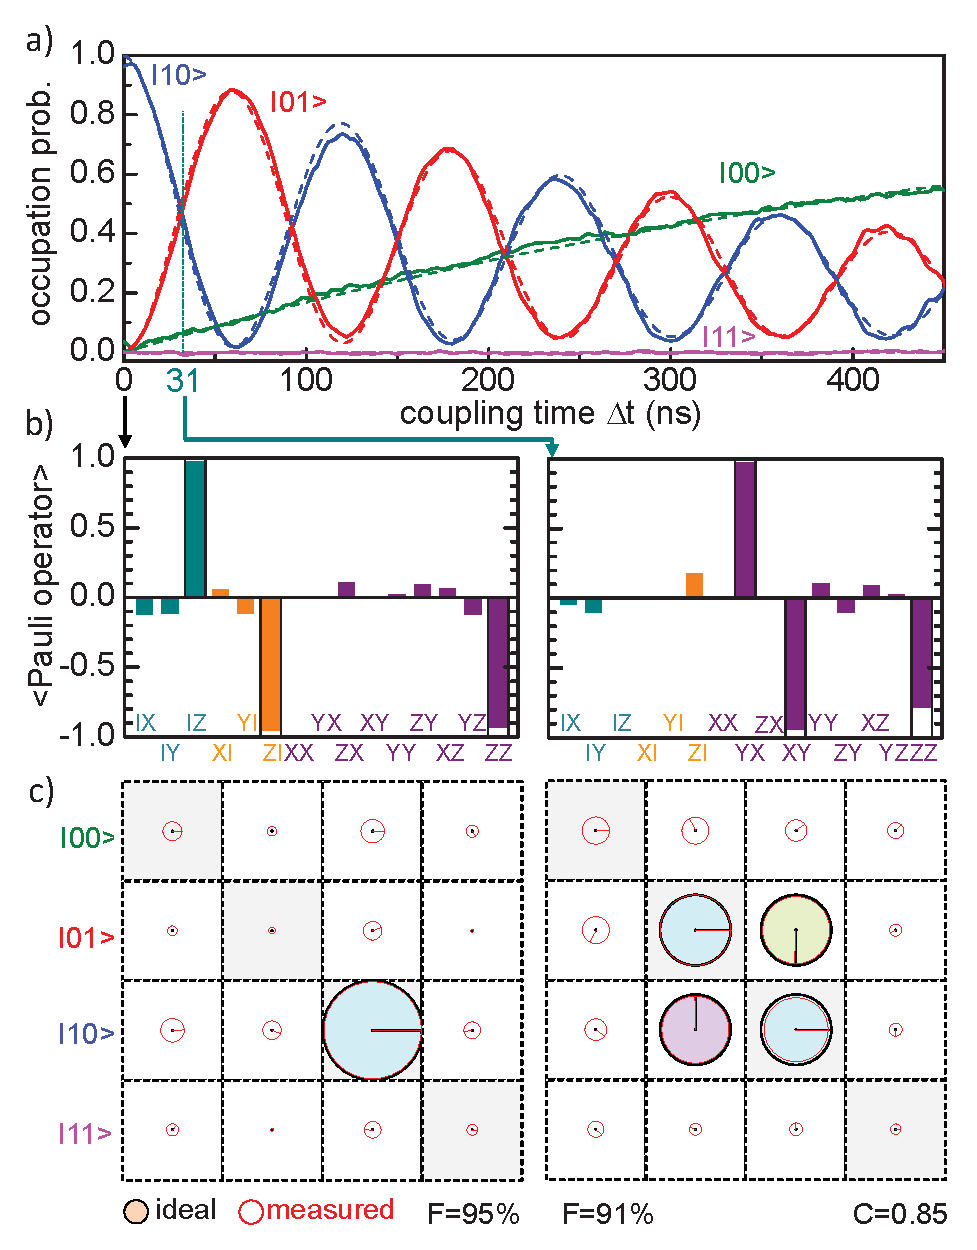
\includegraphics[width=0.7\textwidth]{./material/papers/iswap/submission1/Dewes_Figure2}
\caption[Generating entangled two-qubit states by swapping interaction]{Coherent exchange of a single quantum of excitation
(swapping oscillations) between the two qubits initially prepared
the register state $\left|10\right\rangle $, obtained from the resonant
interaction between them. a) Register state probabilities
as a function of the swapping time $\Delta t$. The frequency of
the oscillations corresponds to $2g/2\pi=8.7\;\mathrm{MHz}$. b) Measured
average values of the Pauli operators products $\left\{ I,\sigma_{x},\sigma_{y},\sigma_{z}\right\} \otimes\left\{ I,\sigma_{x},\sigma_{y},\sigma_{z}\right\} $
(Pauli set) for the register states obtained at times $0\;\mathrm{ns}$
and $31\;\mathrm{ns}$. c) Corresponding reconstructed
density matrices. The area of each circle corresponds
to the absolute value of each matrix element and the color and direction
of the arrow to the phase of the element. The black circles correspond
to the density matrices of the ideal states $\ket{10}$ and $(\ket{10}+i\ket{01})/\sqrt{2}$,
respectively.}


\label{fig:swap_interaction_state_tomography} %
\end{figure}


The capacitive coupling between the two qubits provides a $\sigma_{xx}$-type
interaction that can be used to generate entangled two-qubit states.
Conveniently, this coupling is only effective when the qubit frequencies
are near-resonant and can therefore be effectively switched on and
off by tuning the qubit frequencies in and out of resonance. For the
processor realized in this work, the effective coupling constant $g$
of the two qubits has been measured as $2g/2\pi=8.2\;\mathrm{MHz}$.
When the two qubits are in resonance, the effective evolution operator
of the two-qubit system is:
%
\begin{equation}
U(t)=\left(\begin{array}{cccc}
1 & 0 & 0 & 0\\
0 & \cos{2\pi tg} & i\sin{2\pi tg} & 0\\
0 & i\sin{2\pi tg} & \cos{2\pi tg} & 0\\
0 & 0 & 0 & 1\end{array}\right)_{\left\{ \left|00\right\rangle ,\left|01\right\rangle ,\left|10\right\rangle ,\left|11\right\rangle \right\} } \label{eq:swap_evolution_operator}
\end{equation}
%
 By using fast flux pulses to non-adiabatically tune the qubits in
and out of resonance we can switch on this interaction for a well-defined
time. We first characterize the effect of the coupling on the qubit
register by preparing the state $\ket{10}$, tuning the qubits in
resonance for a given time and measuring the qubit state afterwards.
The resulting curve is shown in fig. \ref{fig:swap_interaction_state_tomography}
and shows swapping oscillations between the two qubits. Analyzing
this curve allows us to extract the effective coupling strength between
them. Leaving the interaction between the qubits on for a well-defined
time allows us to generate entangled Bell states that we characterize
by performing quantum state tomography. The experimental reconstruction
of the density matrix of such a Bell-state of the type $\ket{\psi}=(\ket{01}+i\ket{10})/\sqrt{2}$
is shown in fig. \ref{fig:swap_interaction_state_tomography}b.
The measured fidelity of the prepared state of 91 \% and the concurrence
of 85 \% confirm that entanglement is present in the system. We also
characterize the entanglement between the two qubits by measuring the average value of the so-called \textit{Clauser-Horne-Shimony-Holt}
operator (CHSH) \citep{clauser_proposed_1969}, which
combines measurements of the state of the two qubits along different
axes on the Bloch sphere and provides a test that can distinguish
between classical correlation and quantum entanglement in a two-qubit
system.

%
\begin{figure}[ht!]
 \centering 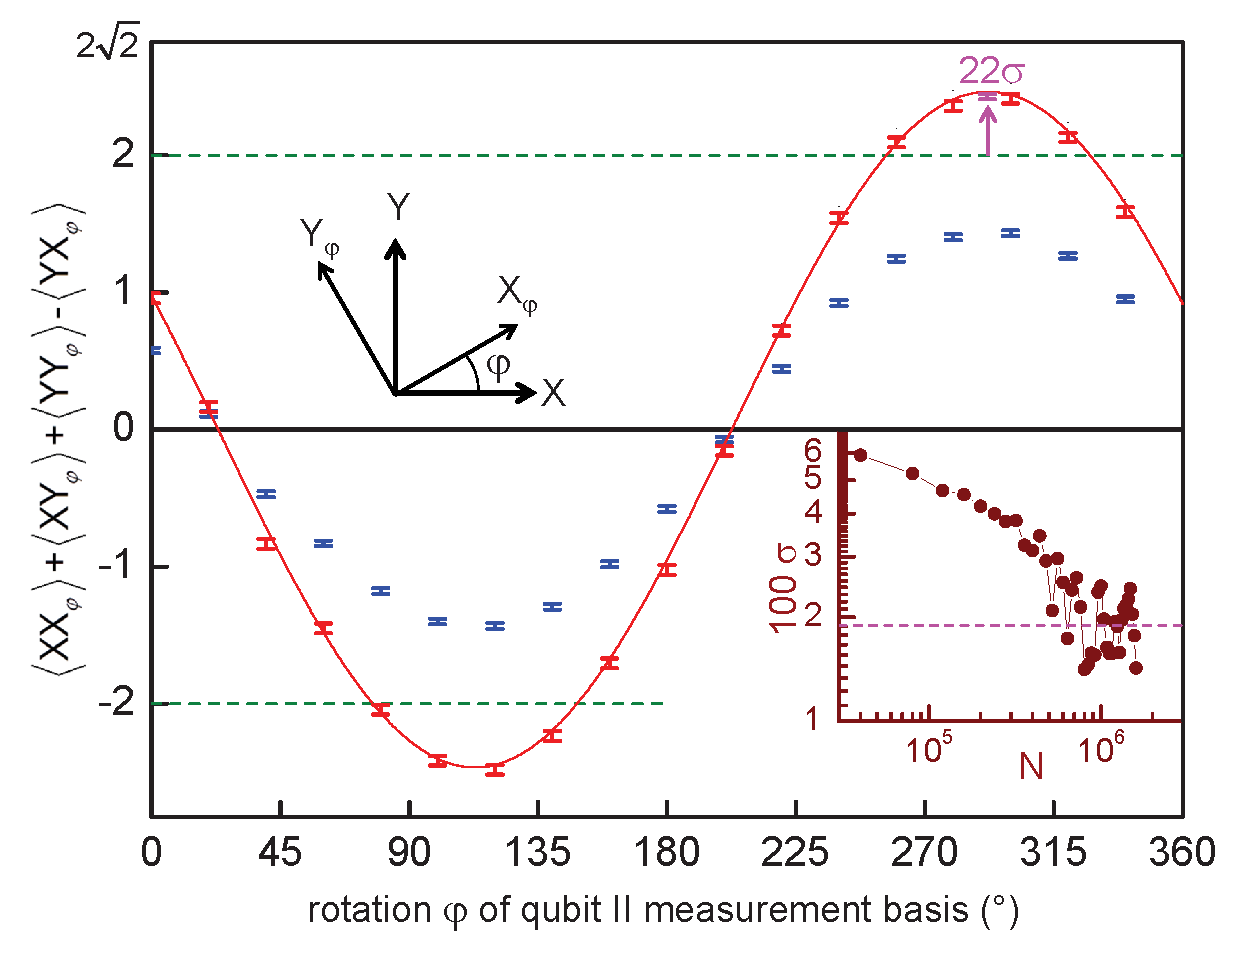
\includegraphics[width=0.7\textwidth]{./material/papers/iswap/submission1/Dewes_Figure3}
\caption[Measurement of the CHSH operator of an entanged two-qubit state]{Measured average value of CHSH operator for a prepared
Bell state. After readout error corrections, the CHSH expectation
value (red points) exceeds the classical boundary of $2$. The raw
measurement data (blue points) lies below this critical threshold.
The inset shows the standard deviation $\sigma$ at the highest point
of the curve as a function of the measurement sample size. For the
highest sample count, the classical boundary is exceeded by $22$
standard deviations.}


\label{fig:chsh_measurement} %
\end{figure}


For classical states, the maximum value of the $\mathrm{CHSH}$ operator
is bound by $2$ but for entangled states it can reach a maximum of
$2\sqrt{2}$. Figure \ref{fig:chsh_measurement}
shows the result of such a $\mathrm{CHSH}$-type measurement performed
on a state created by the method described above, showing the value
of $\bracket{\mathrm{CHSH}}$ as a function of the angle $\phi$ of
the measurement basis. We observe a violation of the classical boundary $2$
of the operator by $22$ standard deviations when correcting the readout
errors that are present in our system. The raw, uncorrected data fails
to exceed the classical threshold because of readout errors mainly
caused by qubit relaxation during the readout. Nevertheless, the observed
violation of the equation in the calibrated data is a strong indication
of entanglement in the system. A more detailed overview of this experiment can be found in chapter \ref{chapter:processor_characterization}.


\section{Realizing a Universal Two-Qubit Quantum Gate}

\begin{SCfigure}[1.0][ht!] 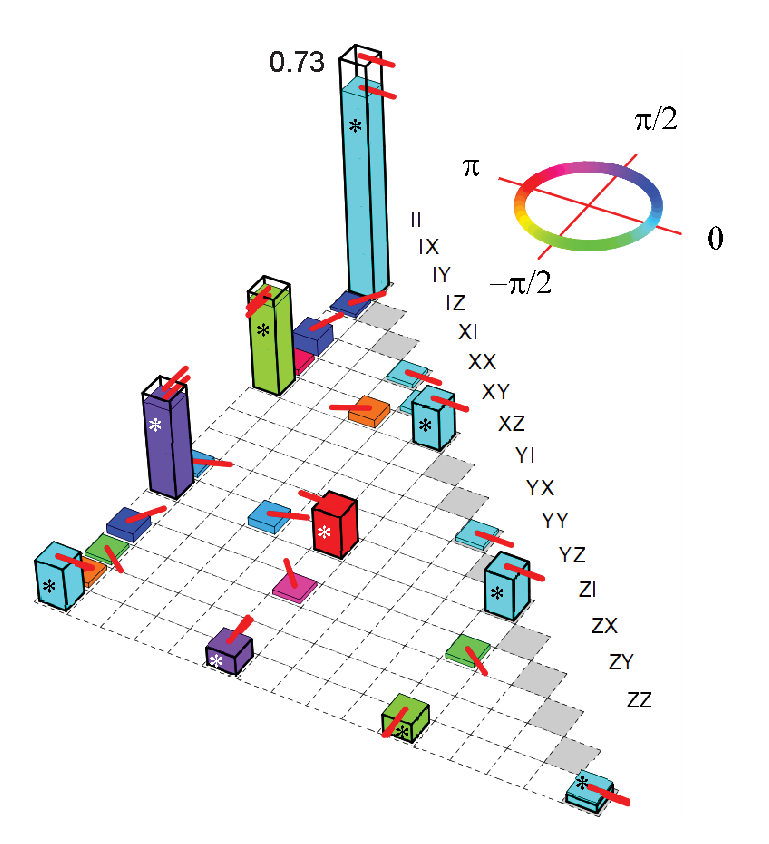
\includegraphics[width=0.65\textwidth]{./material/papers/iswap/figures/chi_matrix}
\caption[Measured $\chi$-matrix of the $\sqrt{i\textrm{SWAP}}$ gate]{Measured $\chi$-matrix of the implemented $\sqrt{i\mathrm{SWAP}}$ gate. The row labels correspond to the indices of the $E_{i}$ Pauli operators, the height of each bar to the absolute value of the corresponding matrix element, and the color and red arrow direction to the argument of the element. The ideal $\chi$-matrix of the $i\sqrt{\mathrm{SWAP}}$ gate is given by the outlined bars. The upper half of the positive-hermitian matrix is not shown.}


\label{fig:gate_chi_matrix_and_errors} \end{SCfigure}

The swapping evolution given by eq. (\ref{eq:swap_evolution_operator})
allows not only to prepare entangled two-qubit states but also to
implement a universal two-qubit gate:
When switching on the interaction for a time $t_{\pi/2}=1/8g$ one
realizes the so-called $\sqrt{i\mathrm{SWAP}}$ gate, represented
by the evolution operator
%
\begin{equation}
U(t)=\left(\begin{array}{cccc}
1 & 0 & 0 & 0\\
0 & 1/\sqrt{2} & i\sqrt{2} & 0\\
0 & i\sqrt{2} & 1/\sqrt{2} & 0\\
0 & 0 & 0 & 1\end{array}\right)_{\left\{ \left|00\right\rangle ,\left|01\right\rangle ,\left|10\right\rangle ,\left|11\right\rangle \right\} } \label{eq:sqrt_iswap_gate}\end{equation}
%
which forms with single qubit gates a universal set
of gates, on which any algorithm can be decomposed. We characterize
the operation and errors of our implementation of this gate by performing
quantum process tomography, obtaining a gate fidelity of 90 \%\ .
The 10 \% error in gate fidelity is caused mainly by qubit relaxation
and dephasing during the gate operation and only marginally by deterministic
preparation errors, as will be discussed in chapter \ref{chapter:processor_characterization}. Figure \ref{fig:gate_chi_matrix_and_errors}
shows the measured $\chi$ matrix of the gate, that describes its
effect in the Pauli basis of two-qubit operators. The $\chi$ matrix
provides the full information on the unitary and non-unitary action
of the gate. The achieved fidelity of the gate operation is sufficient
to allow the implementation of simple quantum algorithms with our
processor.


\section{Running a Quantum Search Algorithm}


The implementation uses a two-qubit quantum gate related to the one
described above to run a simple quantum algorithm on our processor,
the so called \textit{Grover search algorithm} \citep{Grover_Quantum_1997}.
The version of this algorithm that we implement operates on the
two-qubit basis $x_{i}\in\{$ $\ket{00}$ , $\ket{01}$, $\ket{10}$
, $\ket{11}\}$ and can distinguish between four different \textit{Oracle
functions} $\Or_{j}(x)$ with $x\in x_{i}$ that give $\Or_j(x=x_j)=1$ and $\Or_j(x \ne x_j)=0$. In the two-qubit case, this algorithm requires only
one evaluation of the Oracle function $\Or(x)$, implemented as a unitary operator,
to determine which state among the four possible ones it tags. This
case thus provides a simple benchmark of the operation of the quantum
processor, and a simple and illustrative example of quantum speed-up
in comparison with classical algorithms, as discussed
in chapter \ref{chapter:grover_algorithm}. The diagram of the Grover search algorithm implemented
in our processor is shown in fig. \ref{fig:grover_algorithm_schematic_and_density_matrices}a
and involves two $i\mathrm{SWAP}$ gate operations and six single-qubit
operations along with a single-shot qubit readout at the end of the
algorithm. We measured the success probability of the algorithm from
the obtained outcomes, and completed the analysis of its operation
by performing the tomography of the quantum state at different steps
of the algorithm. We first discuss this evolution that sheds light
on how quantum speed-up is achieved.

%
\begin{figure}[ht!]
\centering 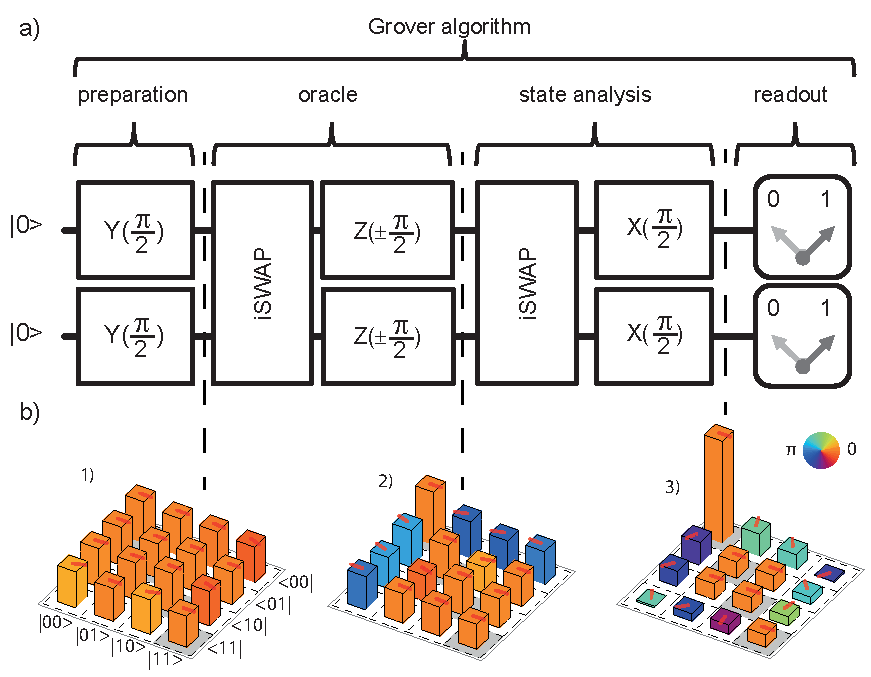
\includegraphics[width=1\textwidth]{material/figures/2-qubit-processor/grover/grover_schematic_and_density_matrices}
\caption[Schematic of the Grover search algorithm and measured density matrices when running it]{a) A two-qubit version of the Grover search algorithm that we implemented on our quantum processor. The algorithm consists in preparing a fully superposed
state, applying a given Oracle operator to it only
once, and analyzing the resulting output to determine the quantum
state tagged by this Oracle operator. b) Measured density matrices when running the Grover search algorithm
with a search oracle marking the state $\ket{00}$. 1) shows the state
after the generalized Hadamard transform, 2) after applying the quantum
oracle and 3) after the final step of the algorithm.}


\label{fig:grover_algorithm_schematic_and_density_matrices} %
\end{figure}


Fig. \ref{fig:grover_algorithm_schematic_and_density_matrices}b
shows the density matrices determined experimentally when running
the Grover search algorithm with the Oracle operator that tags the
state $\ket{00}$. State tomography is first shown after preparation
with a generalized Hadamard transform applied to the initial state
$\ket{00}$. It clearly corresponds then to the superposition of all
the computational basis states, as often done in quantum algorithms. The quantum state after having applied the quantum
Oracle is $-\left|00\right\rangle +\left|01\right\rangle +\left|10\right\rangle +\left|11\right\rangle $
and the information on the tagged state is encoded in the phase of
all matrix elements involving $\ket{00}$ only once. At the end of
the algorithm, the tomography displays a large peak on state $\ket{00}$
, as expected. The fidelity of the final quantum state of the algorithm
is $68\%$, $61\%$, $64\%$ and $65\%$ for the four different Oracle
operators, respectively. These fidelities, corrected for readout errors,
do not quantify the quantum speed-up achieved when running the algorithm. For this, it is necessary to analyze the results obtained
after a single run, which does not allow for any corrections of the
readout outcomes.


\section{Demonstrating Quantum Speed-Up}

%
\begin{figure}[ht!]
 \centering \includegraphics[width=1\textwidth]{"./data/ct5/2011_04_21 - grover and tomo/good_data/grover algorithm - single run probabilities"}
\caption[Single-run results of the Grover search algorithm]{Single-run results when running the Grover search algorithm on our
two-qubit quantum processor. Shown are the probabilities of measuring the qubit register in state $\ket{i}$ for an Oracle function $\Or_j$ marking the state $\ket{j}$
provided to the algorithm. In all four cases, the success probability
of the algorithm is $>50\%$, thus outperforming any classical query-and-guess
algorithm using a single Oracle call.}


\label{fig:grover_single_shot_probabilities} %
\end{figure}


The main interest of running a quantum algorithm is to obtain an advantage
in the run-time in comparision to a classical algorithm, the so-called
\textit{quantum speed-up}. To characterize this speed-up as obtained
with our processor, we run the Grover algorithm for all four possible
Oracle functions and directly read out the state of the qubit register
after the last step of the algorithm instead of performing quantum
state tomography, thus not correcting any readout errors. By averaging
the outcomes of many such individual runs of the algorithm with different
Oracle functions we obtain the so-called \textit{single-run fidelities},
which --for the four different Oracle functions-- have been measured
as $66\%$, $55\%$, $61\%$ and $52\%$. The full probability distributions
for the four possible cases and are shown in fig.
\ref{fig:grover_single_shot_probabilities}. The achieved success
probability is always lower than the theoretically possible value
of 100 \%, mainly because of relaxation and decoherence of the qubit
state during the runtime of the algorithm, and also of errors in the
pulse sequence, but to a small degree. The measured success probabilities
are however larger than the $>50\%$ success probability of a classical
query-and-guess algorithm using the outcome of a single query, which
demonstrates the quantum speed-up achieved with our processor, as
explained in greater detail in the main text. Indeed, a random query-and-guess
allows either to find the searched state, or to rule out one, which
yields to guess the correct answer with $>50\%$ probability instead
of with $>25\%$ for a random guess-and-check. However, since the
gain obtained from a query-and-guess algorithm is not scalable, the
comparison with the $>25\%$ guess-and-check success probability is
more relevant.


\section{Towards a Scalable Multi-Qubit Architecture}

\begin{wrapfigure}[16]{r}{8cm}
	\centering
	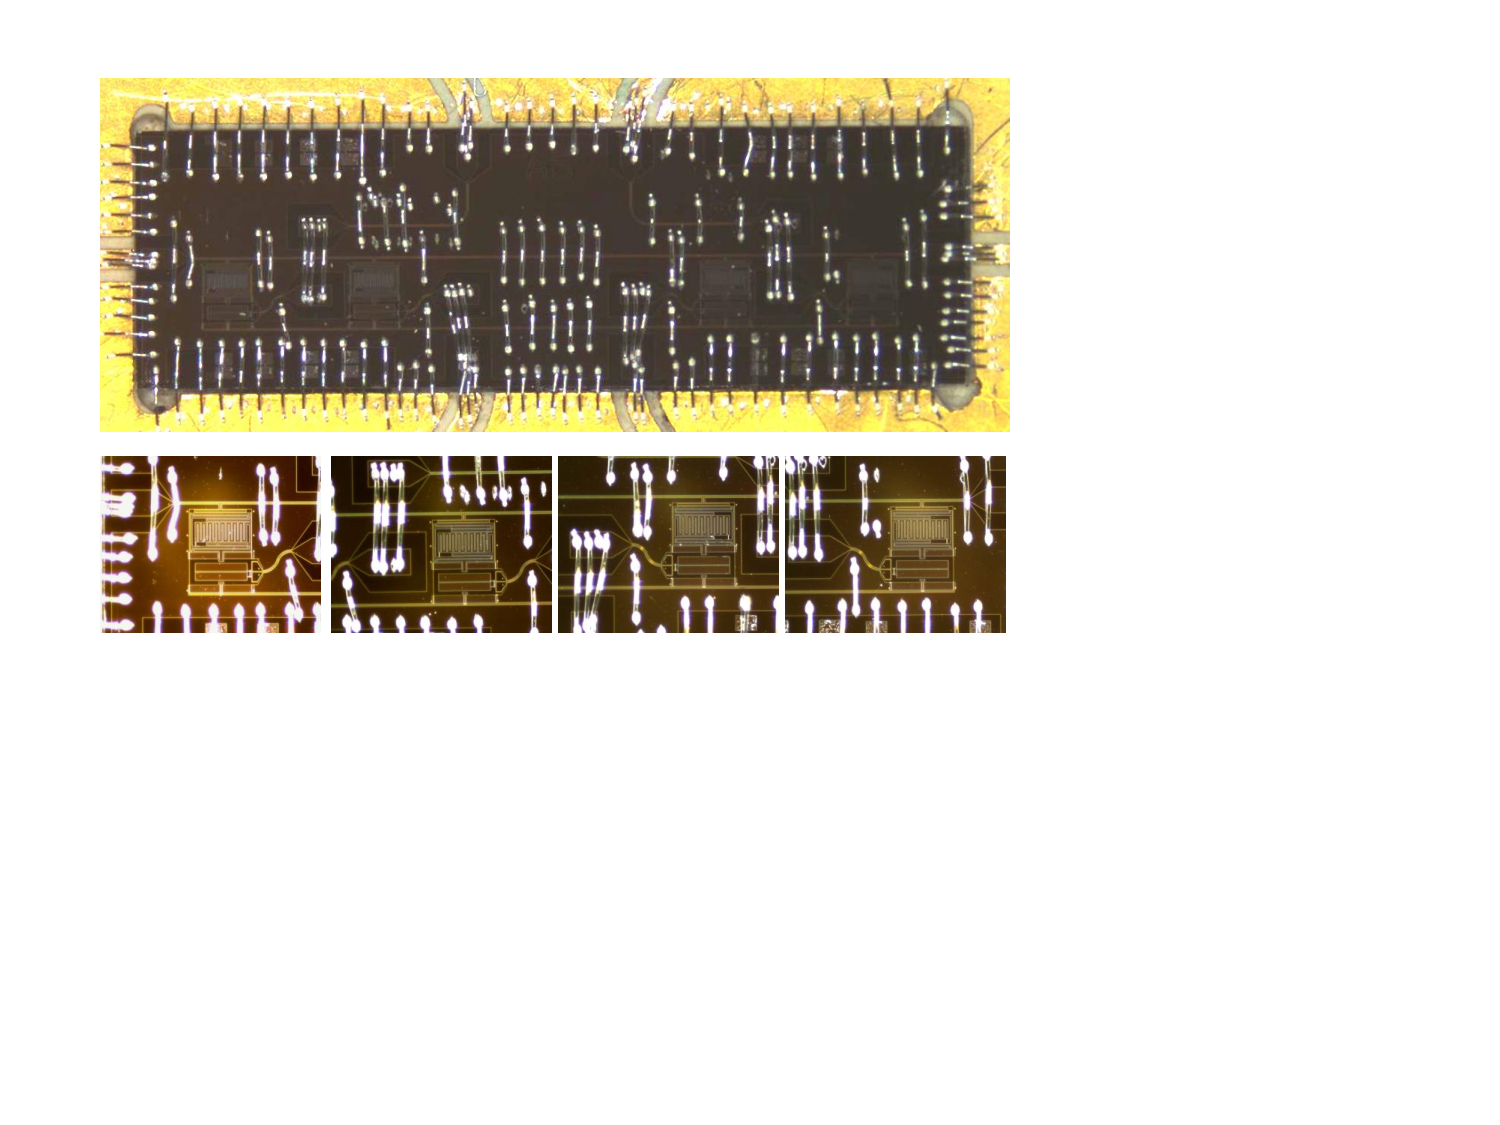
\includegraphics[width=8cm]{./material/figures/scalable-architecture/scalable_architecture_photo}
	\caption[An optical image of the four-qubit chip realized in this work]{An image of the four-qubit chip realized in this thesis work. Shown on top is the whole chip with connectors for the drive and readout transmission line and for the four fast flux lines. The chip is fitted with four qubit/readout cells, each containing a Transmon qubit capacitively coupled to a reaodut resonator and a quantum bus.}
	\label{fig:scalable_architecture_photo}
\end{wrapfigure}

The approach to superconducting quantum computing outlined in the last sections is well suited for the implementation of simple quantum processors with a few qubits. Hovewer, due to several design limitations it is not suitable for implementing a large scale quantum computer. As an example, the direct qubit-qubit coupling employed in this thesis work is not suitable for coupling a large number of qubits since it becomes increasingly difficult to deterministically switch on and off the coupling between individual qubits as the number of qubits increases, a problem sometimes referred to as ``frequency crowding''. Also, fitting each qubit of the processor with individual drive and readout circuitry --as done in this work-- is usually not extensible to a large number of qubits due to topological and space constraints. 

\smallskip

Recently, several research groups have started to address these issues by devising new architectures for superconducting quantum processors that can --in theory-- be scaled to a very large number of qubits. Here we will mention only the so-called ``Rez-Qu'' architecture\citep{galiautdinov_resonatorzero-qubit_2012} and the surface-code approach\citep{divincenzo_fault-tolerant_2009} pursued e.g. by IBM. In this thesis work we discuss our own approach to scalable quantum computing, where we have developed a revised version of our qubit chip that provides a way to implement a system with a larger --albeit still small-- number of qubits. Key elements of this architecture are a quantum bus in form of a high-Q microwave resonator that is used for coupling the qubits and a multiplexed drive and readout circuit that allows us to measure and manipulate all qubits through one single microwave transmission line. 

Figure \ref{fig:scalable_architecture_photo} shows an optical image of the first version of this architecture. Our chip contains four Transmon qubits which are capacitively coupled to a distributed high-Q resonator acting as a quantum bus. In addition, each qubit is coupled to a low-Q lumped element resonator that is used for reading out the qubit state. Each of these resonators is in turn coupled capacitively to the input transmission line. The resonance frequencies of the readout resonators are arranged in ascending order with a frequency spacing of $\approx 150\;\mathrm{MHz}$ between adjacent resontaors. This frequency spacing allows us to address each resonator individually and to read out the state of the full qubit register in parallel using only one single transmission line. Fig. \ref{fig:jba_multiplexed_spectroscopy} shows the measured $|S_{01}|$ matrix element of such a chip with four JBA resonators at frequencies between 6.78 GHz and 6.95 GHz, plotted as a function of the incident microwave power. The ``knee'' in each of the four resonance curves appearing between -45 and -40 dBm corresponds to the bifurcation point of the resonators.

\begin{wrapfigure}[30]{r}{8cm}
	\centering
	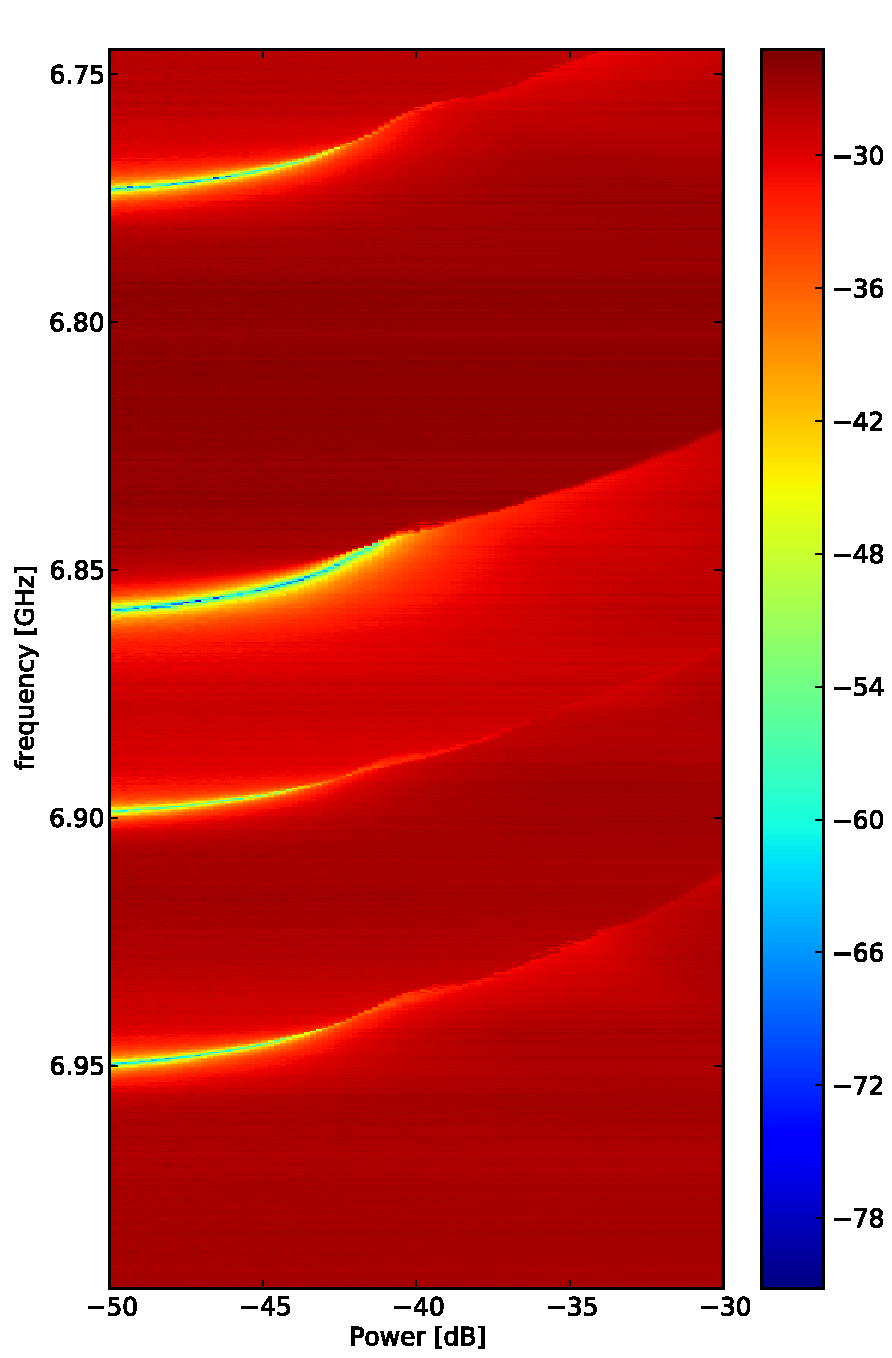
\includegraphics[width=8cm]{./material/figures/scalable-architecture/jba_multiplexed_spectroscopy}
	\caption[Measured $|S_{10}|$ transmission coefficient for the input transmission line of our four-qubit chip]{The measured $|S_{10}|$ tranmission coefficient for the input transmission line of our four-qubit chip. Clearly visible are four resonances of the JBA resonators and the bifurcation of each resonator at high input power.}
	\label{fig:jba_multiplexed_spectroscopy}
\end{wrapfigure}

Still, this approach suffers from a relatively bad ON/OFF ration in the qubit-qubit coupling. To alleviate this problem, the Transmon qubit used in the current version of this architecture can be replaced by a qubit with a tunable coupling\citep{srinivasan_tunable_2011}. Alternatively, it is possible to use a fixed-frequency coupling scheme for the qubits, thereby altogether eliminating the need for frequency tuning of individual qubits and also reducing the number of input transmission lines form $n+1$ to $1$.

\smallskip

A detailed discussion of the scalable architecture and the first preliminary measurements performed with a four-qubit chip will be presented in chapter 7 of this thesis.